\chapter{Intersection}

Given an implicit surface equation $ f\left( x, y, z \right) = 0 $, we
want to find a point $ p $ that is on the surface,
i.e. $ f\left( p \right) = 0 $. Since $ p = O + dt $, we are looking for
$ t $ in $ f\left( O + td \right) = 0 $.

If $ t < 0 $, then intersection is behind the screen

\textbf{Robustly}: a solution is resistant to error and produces similar
result for small changes in input

\section{Axis Aligned Bounding Boxes (AABB)}

  Slabs are the differences between the min and max $ x, y, z $ values.
  A ray misses the box if the slab intersection intervals do not
  overlap.

  Check if the entering $ t $ is smaller than the smallest exiting $ t $

  \begin{figure}[H]
    \centering
    \caption{Axis Aligned Bounding Boxes Hit Test}
    \includegraphics[width=\columnwidth]{images/intersection/aabb-hit-test.png}
  \end{figure}

\section{Plane}

  \begin{align}
    Ax + By + Cz + D &= 0 \\
    \left( p - a \right) \cdot n = 0
  \end{align}

  $ a $ is a \textbf{point in space} and $ n $ is the \textbf{normal vector}
  of the plane with its origin at $ a $

  Given a ray $ O + td $ we can solve for a $ t $, which gives us the
  point of intersection.

  \begin{align*}
    \left( p - a \right) \cdot n &= 0 \\
    \left( \left( O + td \right) - a \right) \cdot n &= 0 \\
    \frac{\left( \left( a - O \right) \cdot n \right)}{d \cdot n} &= t
  \end{align*}

  \begin{itemize}
    \item If the ray and the plane is parallel, then $ d \cdot n = 0 $
    \item If the intersection is behind the origin then $ t < 0 $
  \end{itemize}

\section{Sphere}

  Spheres are defined by

  \begin{equation}
    \left( P - G \right) \cdot \left( P - G \right) = r^{2}
  \end{equation}

  $ P $ is a \textbf{point is space}, $ G $ is the \textbf{center of sphere},
  and $ r $ is the \textbf{radius of sphere}

  Replace $ P $ with $ O + td $ and let $ f = O - G  $

  \begin{align}
    \left( d \cdot d \right) t^{2}
      + 2 \left( f \cdot d \right) t
      + f \cdot f - r^{2}
    &= 0 \\
    a t^{2} + bt + c &= \\
    \frac{-b \pm \sqrt{b^{2} - 4ac}}{2a} &= t_{0, 1} \\
    \frac{P_{0} - G}{r} &= n
  \end{align}

  \begin{itemize}
    \item $ t_{0, 1} $: rays will have two intersection points
    \item $ b^{2} - 4ac < 0 $: ray does not intersect with sphere
    \item $ b^{2} - 4ac > 0 $: ray intersects with sphere
    \item $ b^{2} - 4ac = 0 $: ray touches sphere on the surface
  \end{itemize}

  \subsection{Diminished Significance}

    \paragraph{Problem}
    \begin{itemize}
      \item 32 bit float point can result in error; caused by
      \textbf{diminished} significance
      \begin{itemize}
        \item Ex. small spheres that are very far away
      \end{itemize}

      \item $ c = f \cdot f - r^{2}  $ is problematic, if $ f $ is big and $ r $ is
      small, diminished significance would occur. If a sphere is more than
      \begin{equation}
        2^{12} r = 4096 r
      \end{equation}
      away from the ray origin, then radius has no impact on intersection
      solution.
    \end{itemize}

    \paragraph{Solution} \textbf{Hearn Baker Method}
    \begin{align}
      b^{2} - 4ac &= 4a \left( \frac{b^{2}}{4a} - c \right) \\
      &= 4d^{2} \left( r^{2} - \left( f - \left( f \cdot \hat{d} \right) \hat{d} \right)^{2} \right)
    \end{align}

  \subsection{Catastrophic Cancellation}

    \paragraph{Problem}
    \begin{itemize}
      \item Occurs when adding nearly equal numbers with opposite signs.
      In sphere intersection, it occurs in
      \begin{equation*}
        -b \pm \sqrt{b^{2} - 4ac}
      \end{equation*}

      when

      \begin{equation*}
        b \approx \sqrt{b^{2} - 4ac}
      \end{equation*}

      \item Many significant bits eliminate each other
      \item Few meaningful bits remain
    \end{itemize}

    We have approximations

    \begin{align}
      \tilde{x} &= x \left( 1 + \delta_{x} \right) \\
      \tilde{y} &= y \left( 1 + \delta_{y} \right)
    \end{align}

    Small relative errors

    \begin{align}
      \left| \delta_{x} \right| &= \frac{\left| x - \tilde{x} \right|}{\left| x \right|} \\
      \left| \delta_{y} \right| &= \frac{\left| y - \tilde{y} \right|}{\left| y \right|}
    \end{align}

    Relative error of the difference can be arbitarrily large

    \begin{equation}
      \left| \frac{x \delta_{x} - y \delta_{y}}{x - y} \right|
    \end{equation}

    \paragraph{Solution} Catastrophic cancellation only happens to one of the
    two quadratic solutions. Can be fixed using $ t_{0} t_{1} = \frac{c}{a} $

    \begin{equation}
      \begin{cases}
        t_{0} = \frac{c}{q} \\
        t_{1} = \frac{q}{a}
      \end{cases}
    \end{equation}

    where $ q = \frac{1}{2}\left( b + \sign\left( b \right) \sqrt{b^{2} - 4ac} \right) $
    $ \sign $ function returns 1 if $ b > 0 $ and $ - 1 $ otherwise

\section{Triangles}

  \subsection{Barycentric Coordinates}

    Barycentric coordinates can be used to

    \begin{itemize}
      \item Determine if a ray hits a triangle
      \item Determine the color of a point in a triangle by interpolating from
      the colors of three vertices
    \end{itemize}

    Barycentric coordinates can be used on any \gls{simplex}.
    A \textbf{\gls{simplex}} is a \glsdesc{simplex}.

    Barycentric coordinates describes the location of a point in relation to
    the vertices of a given triangle:
    $ p_{b} = \left( b_{1}, b_{2}, b_{3} \right) $

    \begin{align}
      p_{w} &= b_{1} a + b_{2} b + b_{3} c \\
      1 &= b_{1} + b_{2} + b_{3} \\
      f\left( p \right) &=
        b_{1} f\left( a \right)
        + b_{2} f\left( b \right)
        + b_{3} f\left( c \right)
    \end{align}

    \begin{itemize}
      \item $ p_{b} $ is a point in triangle in barycentric coordinate
      \item $ p_{w} $ i a point in triangle in world coordinate
      \item $ f\left( x \right) $ is the value of a point in triangle, $ x $
    \end{itemize}

    Coordinates are the \textbf{signed} area of the opposite subtriangle
    divided by the area of the triangle.

    \begin{itemize}
      \item For a point in the triangle, all barycentric values are not negative
    \end{itemize}

    \begin{align}
      b_{x} = \frac{\area\left( T_{x} \right)}{\area\left( T \right)}
    \end{align}

    \begin{figure}[H]
      \centering
      \caption{2D Barycentric Coordinates}
      \includegraphics[width=0.7\columnwidth]{images/intersection/2d-barycentric.png}
    \end{figure}

    \begin{itemize}
      \item $ p_{x}, p_{y} $ is a point in the triangle
      \item $ x_{i}, y_{i}, z_{i} $ is a vertex $ i $ of the triangle
      \item $ b_{i} $ is the barycentric coordinates
    \end{itemize}

    \begin{figure}[H]
      \centering
      \caption{3D Barycentric Coordinates}
      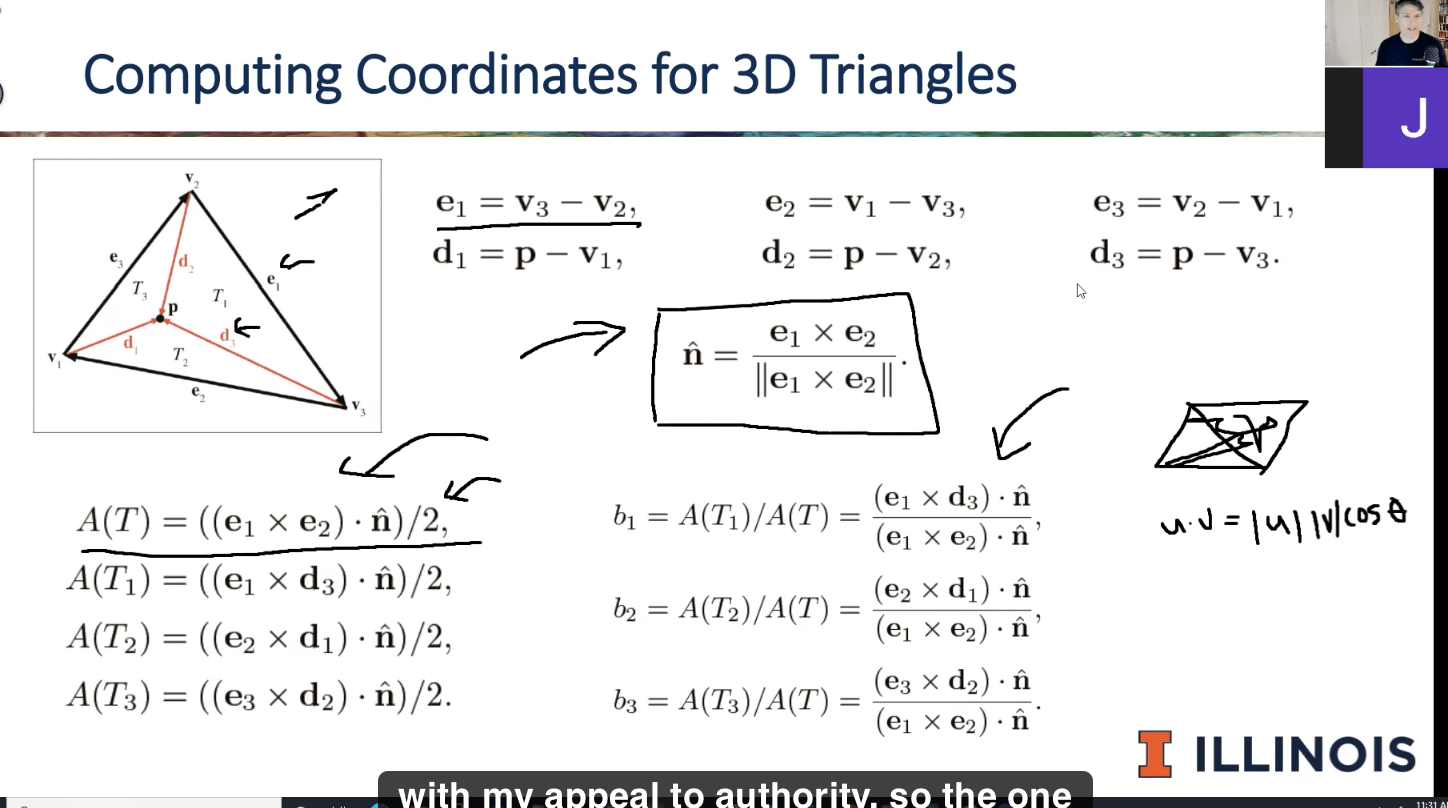
\includegraphics[width=0.7\columnwidth]{images/intersection/3d-barycentric.png}
    \end{figure}

    The above 3D barycentric coordinates works in both left and right handed
    coordiante systems (normals in the above calculation do not; have to
    flip the direction of all the vectors)

  \subsection{Intersection}

    \begin{align}
      O + t d &= \left( 1 - u - v \right) p_{0} + u p_{1} + v p_{2} \\
      O - p_{0} &=
      \begin{bmatrix}
        -d & p_{1} - p_{0} & p_{2} - p_{0}
      \end{bmatrix}
      \begin{bmatrix}
        t \\
        u \\
        v
      \end{bmatrix}
    \end{align}

    \begin{itemize}
      \item $ u, v, \left( 1 - u - v \right) $ is the barycentric coordiante
      of the intersection point
      \item $ p_{x} $ are the vertices of the triangle
      \item Solving this system using Cramer's rule takes
      $ O\left( n! n \right) $ and using Gaussian rule takes
      $ O\left( n^{3} \right) $
      \item Cramer's rule is not as stable as Gaussian's rule
    \end{itemize}

    \begin{figure}[H]
      \centering
      \caption{Triangle Intersection using Cramer's Rule}
      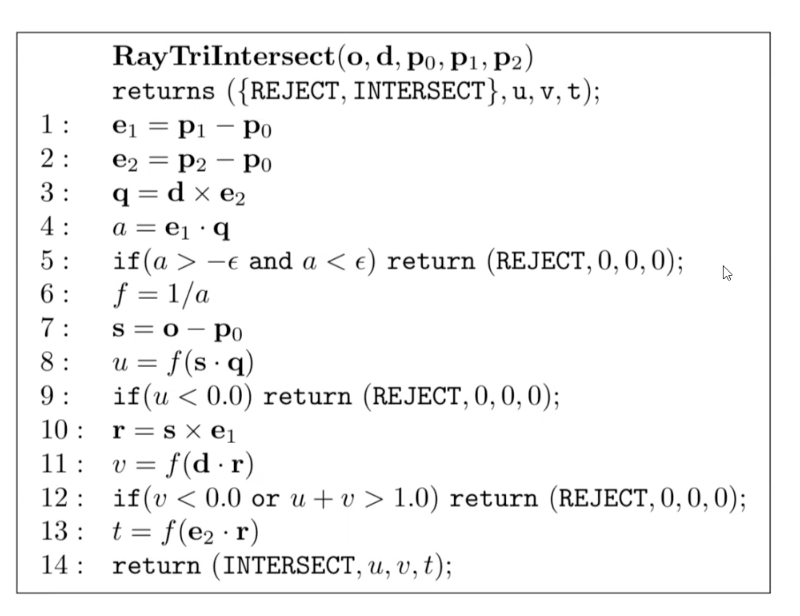
\includegraphics[width=0.7\columnwidth]{images/intersection/triangle-hit-test.png}
    \end{figure}

    \begin{itemize}
      \item $ e = 10^{-5} $ is a good choice
      \item Line 4 computes the determinant of matrix $ M $; then test
      to avoid determinants close to zero
    \end{itemize}

\section{Parabolic Cylinder}

  Parabolic cylinder is defined by

  \begin{equation}
    z = x^{2}
  \end{equation}

  Using

  \begin{align*}
    p_{x} &= O_{x} + t d_{x} \\
    p_{z} &= O_{z} + t d_{z}
  \end{align*}

  Parabolic cylinder can be redefined as

  \begin{align*}
    O_{z} + t d_{z} &= O_{x}^{2} + 2 O_{x} t d_{x} + t^{2} d_{x}^{2} \\
    0 &= d_{x}^{2} t^{2} + t \left( 2 O_{x} d_{x} - d_{z} \right)
      + \left( O_{x}^{2} - O_{z} \right) \\
      &= a t^{2} + bt + c
  \end{align*}

  Which is a quadratic equation

\section{Dealing With Transformations}

  \begin{enumerate}
    \item Apply inverse transformation to the ray
    \item Intersect the transformed ray with untransformed object
    \item Compute normal at hit point
    \item Use hit point to compute hit point on transformed object
    \item Use normal to compute normal on transformed object
    \begin{equation}
      n' = \left( T^{-1} \right)^{T} n
    \end{equation}
    \begin{itemize}
      \item Same as in rasterization
    \end{itemize}
  \end{enumerate}

  \subsection{Instancing}

    \begin{itemize}
      \item Keep a single original model
      \item Create instance models which
      \begin{itemize}
        \item Reference original model
        \item Inverse transformation matrix
        \item Material
      \end{itemize}
    \end{itemize}

  \subsection{Bounding Box}

    \begin{itemize}
      \item Apply transformations to the corners bounding box
      \item Recompute min and max
    \end{itemize}
